\documentclass[12pt,a4paper]{ctexart}

\usepackage[a4paper,margin=2.5cm]{geometry}
\usepackage{setspace}
\usepackage{array}
\usepackage{longtable}
\usepackage{graphicx}
\usepackage{fancyhdr}
\usepackage{titling}
\usepackage{enumitem}
\usepackage{amsmath,amssymb}
\usepackage{booktabs}
\usepackage{caption}
\usepackage{float}
\usepackage{bm}
\usepackage{hyperref}
\usepackage{listings}
\usepackage[dvipsnames, svgnames, x11names]{xcolor}

\lstset{ 
	backgroundcolor=\color[rgb]{0.96,0.96,0.96},% 背景颜色
	keywordstyle=\color{blue}\bfseries,         % 关键字颜色
	identifierstyle=\color{black},              % 普通标识符颜色
	commentstyle=\color[rgb]{0,0.6,0},          % 注释颜色
	stringstyle=\color[rgb]{0.58,0,0.82},
	basicstyle=\small\ttfamily,        % size of fonts used for the code
	columns=fullflexible,
	breaklines=true,                 % 自动换行
	captionpos=t,                    % sets the caption-position to bottom
	tabsize=4,
	%escapeinside={\%*}{*)},          % if you want to add LaTeX within your code
	morekeywords={}, % 设置更多的关键字，用逗号分隔
	emph={self}, % 指定强调词，如果有多个，用逗号隔开
	emphstyle=\bfseries\color{Rhodamine}, % 强调词样式设置
	frame=lines, % 边框
	framesep=1em, % 设置代码与边框的距离
	rulesepcolor=\color{red!20!green!20!blue!20},
	language=C++,
	numbers=left, % 显示行号在左边
	showstringspaces=false,                     % 不显示字符串内的空格
	%	numbersep=2em, % 设置行号的具体位置
	numberstyle=\footnotesize, % 缩小行号
	extendedchars=false,
	xleftmargin=3em
}

\setlength{\parindent}{2em}
\setlength{\parskip}{0.5em}
\renewcommand{\arraystretch}{1.5}
\linespread{1.3}

\pagestyle{fancy}
\fancyhf{}
\cfoot{\thepage}
\renewcommand{\headrulewidth}{0pt}


% ===== 可修改信息 =====
\newcommand{\schoolname}{数学与统计学院}
\newcommand{\classname}{数学强基2301}
\newcommand{\studentid}{2233210080}
\newcommand{\studentname}{袁浩然}
\newcommand{\teachername}{孟德宇老师}
\newcommand{\labplace}{数学实验中心}
\newcommand{\experimenttitle}{BP 算法解决二分类问题}
\newcommand{\schoolyear}{2023--2024学年\quad 第二学期}\usepackage{fancyhdr}

% 设置 fancyhdr 样式
\fancypagestyle{plain}{
	\fancyhf{} % 清除所有预设的页眉和页脚
	\renewcommand{\headrulewidth}{0pt} % 如果不需要页眉线
	\renewcommand{\footrulewidth}{0pt} % 如果不需要页脚线
}

% 应用新的 plain 样式到所有页面
\pagestyle{plain}

\begin{document}

	\section*{BP 算法解决二分类问题}
	%\experimentname
	
	\section*{一、实验内容}
	本次实验我们尝试使用利用前馈神经网络解决 XOR 问题。我们搭建一个带单隐层的神经网络，用 BP（反向传播）算法完成参数更新，让网络能够把四组输入
	\[
	X = \{[0,0],[0,1],[1,0],[1,1]\}
	\]
	对应到标签
	\[
	Y = \{0,1,1,0\}
	\]
	上。这个任务数据量不大，但是正好能说明一个问题：像 XOR 这种线性不可分的数据，单层线性模型是处理不了的，必须通过隐藏层引入非线性变换。
	
	本次实验我们的任务流程如下所示：我们规定迭代次数为600次，并使用 Adam 作为我们的优化器，选取学习率为 $0.01$ ，另外，我们选取 MSE 作为损失函数，对最终结果进行优化更新，另外，我们的神经网络架构如下所示：我们引入 torch 的 nn.Module 板块，设置输入层与输出层如下下所示：
\begin{lstlisting}
self.layer1 = nn.Linear(3, 5)
self.lyaer2 = nn.Linear(5, 1)
\end{lstlisting}
并选取 Sigmoid 函数作为激活函数：
$$\sigma(x)=\dfrac{1}{1+e^{-x}}$$
我们设置 batch\_size=4 ，并得到了最后的网络架构。 

	\section*{神经网络简介}
	
	\subsection*{介绍}
	神经网络中的结构如下所示，并且他有着这样的解释：
	\begin{enumerate}
		\item 设计一个神经网络时，输入层与输出层的节点数往往是固定的，中间层则可以自由指定；
		\item 神经网络结构图中的拓扑与箭头代表着预测过程时数据的流向，跟训练时的数据流有一定的区别
		\item 结构图里的关键不是圆圈（代表“神经元”），而是连接线（代表“神经元”之间的连接）。每个连接线对应一个不同的权重（其值称为权值），这是需要训练得到的。 
	\end{enumerate}
	\begin{figure}[H]
		\centering
		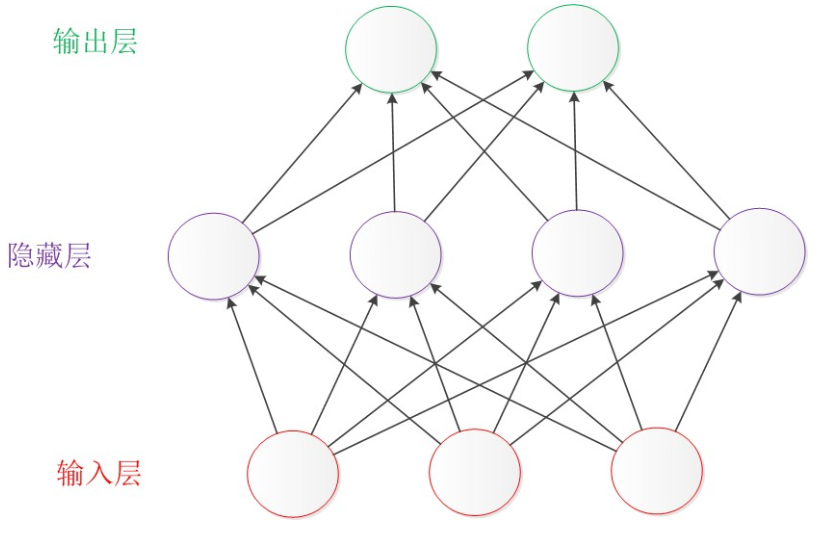
\includegraphics[scale=0.4]{从下到上的神经网络图.png}
	\end{figure}
	
	\subsection*{神经元}
	神经元模型是一个包含输入、输出和计算功能的模型，这里输入类比为树突，输出看成是轴突，计算可以类比为细胞核，其中计算可以被分为加权和非线性映射。
	\begin{figure}[H]
		\centering
		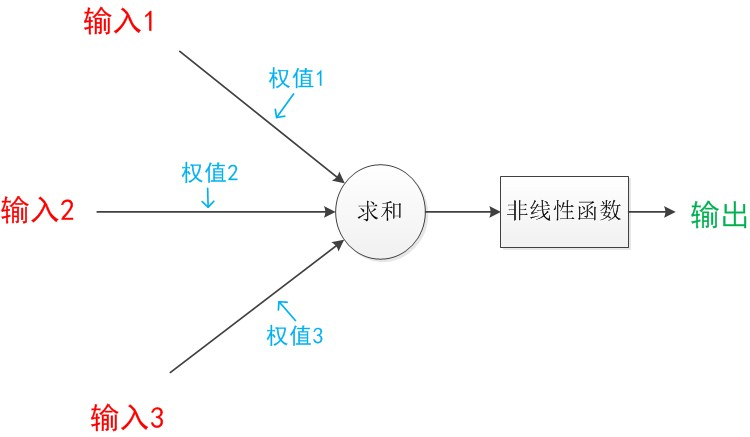
\includegraphics[scale=0.3]{神经元模型.png}
	\end{figure}
	
	\subsection*{单层神经网络 (感知器)}
	当一个神经元的输出可以向多个神经元传递，则我们就产生了单层神经网络，我们可以用下面这张图来表示单层神经网络：
	\begin{figure}[h]
		\centering
		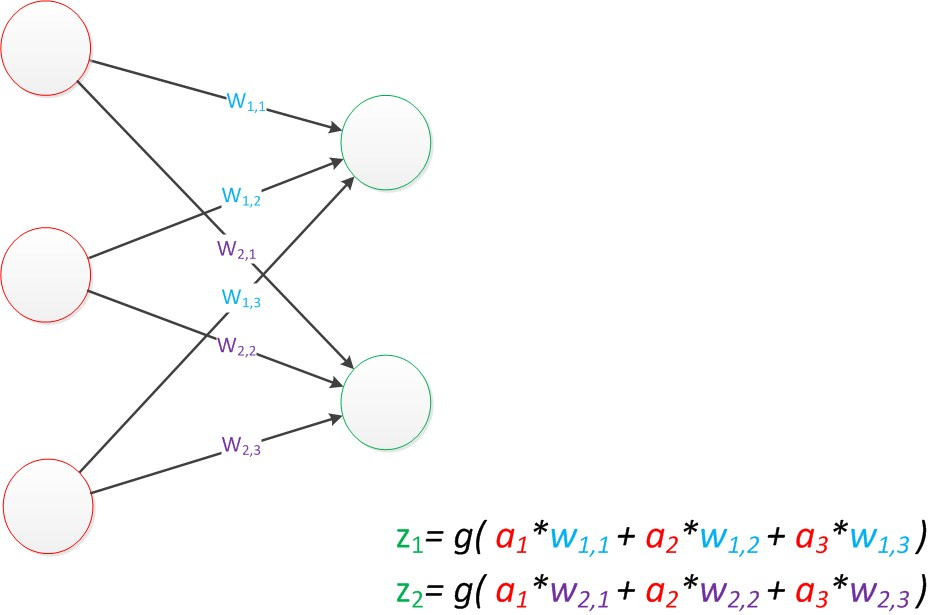
\includegraphics[scale=0.2]{单层神经网络.png}
	\end{figure}
	如果我们用 $\bm{x}=[a_1,a_2,a_3]^T$ 表示输入, $\bm{z}=[z_1,z_2]^T$ 表示输出，并且将系数写作矩阵的形式 $W$ ,则有输出公式
	$$\bm{z}=g(W\bm{a})$$
	
	\subsection*{两层神经网络 (多层感知器)}
	\subsubsection*{基本概念}
	两层神经网络除了包含一个输入层，一个输出层以外，还增加了一个中间层。此时，中间层和输出层都是计算层。我们扩展上节的单层神经网络，在右边新加一个层次。
	\begin{figure}[H]
		\centering
		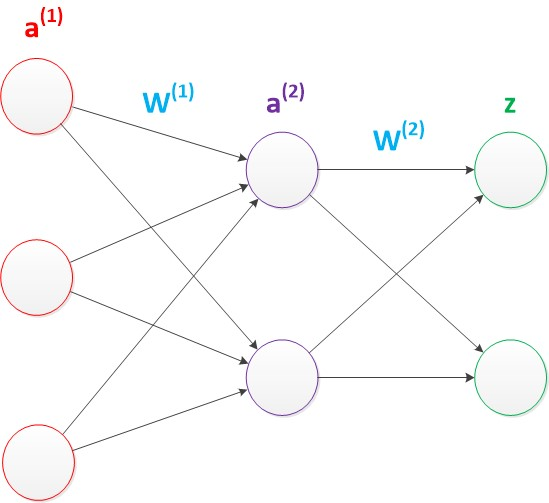
\includegraphics[scale=0.2]{两层神经网络.png}
	\end{figure}
	我们用举着你形式来表示上面的神经网络：
	$$g(W^{(1)}\bm{a}^{(1)})=\bm{a}^{(2)}$$
	$$g(W^{(2)}\bm{a}^{(2)})=\bm{z}$$
	在单层神经网络中，我们一般使用 sgn 函数来作为非线性函数，而对于两层神经网络，我们选择 sigmoid 作为函数 $g$ 。这里我们基于损失函数与梯度下降对权重进行训练，我们使用一定量的数据集，并对神经网络中的所有参数赋上随机值，我们采用求导的形式对我们使用的损失函数，一般是平方损失函数：
	$$\text{loss}=||y-y_{p}||^2$$
	对每个参数采用梯度下降法，找到最优解，这便对神经网络完成了训练。
	
	\subsection*{多层神经网络}
	对于两层神经网络，我们可以再增加几个中间层，进而就得到了多层神经网络。
	\begin{figure}[H]
		\centering
		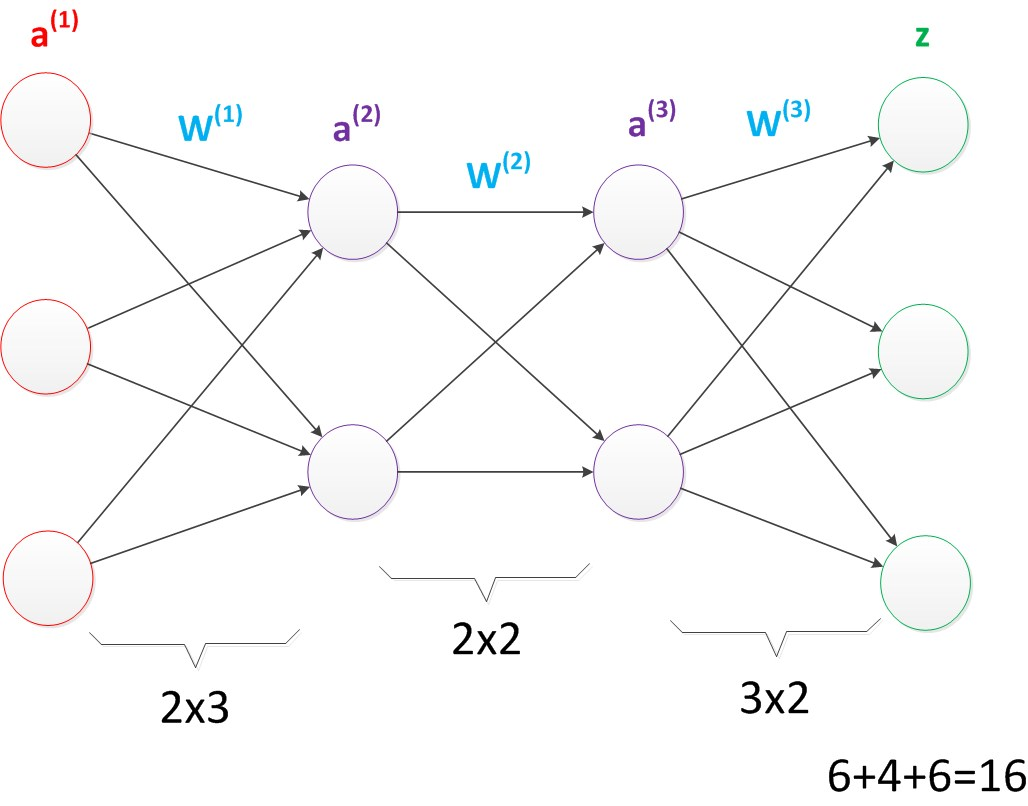
\includegraphics[scale=0.15]{多层神经网络.png}
	\end{figure}
	更深入的表示特征可以这样理解，随着网络的层数增加，每一层对于前一层次的抽象表示更深入。在神经网络中，每一层神经元学习到的是前一层神经元值的更抽象的表示。例如第一个隐藏层学习到的是“边缘”的特征，第二个隐藏层学习到的是由“边缘”组成的“形状”的特征，第三个隐藏层学习到的是由“形状”组成的“图案”的特征，最后的隐藏层学习到的是由“图案”组成的“目标”的特征。通过抽取更抽象的特征来对事物进行区分，从而获得更好的区分与分类能力。
	
	在多层神经网络中，我们一般采用 ReLU 函数作为非线性函数，其更容易收敛，并且预测性能较好。对于训练，我们采用的方式仍然是优化和泛化。
	
	\section*{三、关于反向传播算法}
	
	
	\section*{四、问题描述与原理}
	XOR 的特点是：两个输入不同时输出 1，相同时输出 0。它看起来很简单，但不能直接用一条直线分开，所以很适合作为 BP 神经网络的入门例子。
	
	我这里使用的是一个三层结构的网络：输入层、单隐层和输出层。因为代码里额外拼接了一列常数 1 来模拟偏置，所以输入维度实际按 3 维处理。隐藏层有 5 个神经元，激活函数采用 sigmoid，输出层输出 1 个值。损失函数用的是均方误差（MSE），优化器使用 Adam。
	
	整个前向传播过程可以写成：
	\[
	H = \sigma(XW_1 + b_1), \qquad \hat{Y} = HW_2 + b_2
	\]
	其中 $\sigma(\cdot)$ 表示 sigmoid 函数。训练时通过反向传播计算梯度，再不断更新参数，使预测值 $\hat{Y}$ 逐步接近真实标签 $Y$。
	
	\section*{四、实验步骤}
	\begin{enumerate}
		\item 构造 XOR 数据集，并把输入和标签都转成张量；
		\item 为了方便处理偏置，在输入后额外拼接一列常数 1；
		\item 定义网络结构：输入层 3 维，隐藏层 5 维，输出层 1 维；
		\item 编写前向传播函数，隐藏层使用 sigmoid 激活；
		\item 设定损失函数为 MSELoss，优化器为 Adam，学习率设为 0.01；
		\item 训练 600 轮，并记录每轮的损失值；
		\item 在训练结束后，对四组 XOR 输入进行预测，并将结果可视化展示。
	\end{enumerate}
	
	\section*{五、核心代码}
	下面是本次实验使用的主要代码。为了和运行结果保持一致，这里保留了我实际写程序时的网络结构和训练参数。
	
	\begin{lstlisting}
import torch
import torch.nn as nn
from torch.utils.data import DataLoader, TensorDataset
import matplotlib.pyplot as plt

EPOCH = 600
LR = 0.01

device = torch.device("cuda" if torch.cuda.is_available() else "cpu")
print(f"Using device: {device}")

x_all = torch.tensor([[0, 0], [0, 1], [1, 0], [1, 1]], dtype=torch.float32).to(device)
y_all = torch.tensor([[0], [1], [1], [0]], dtype=torch.float32).to(device)

dataset = TensorDataset(x_all, y_all)
dataloader = DataLoader(dataset, batch_size=4, shuffle=True)

class LinearModel(nn.Module):
	def __init__(self):
		super().__init__()
		self.layer1 = nn.Linear(3, 5)
		self.layer2 = nn.Linear(5, 1)
	
	def forward(self, x):
		tmp = torch.sigmoid(self.layer1(x))
		return self.layer2(tmp)

model = LinearModel().to(device)
criterion = nn.MSELoss()
optimizer = torch.optim.Adam(model.parameters(), lr=LR)
loss_history = []

for epoch in range(EPOCH):
	for x_batch, y_batch in dataloader:
		x_batch = torch.cat((x_batch, torch.ones(x_batch.size(0), 1).to(device)), dim=1)
		y_pred = model(x_batch)
		loss = criterion(y_pred, y_batch)
		optimizer.zero_grad()
		loss.backward()
		optimizer.step()
	
		loss_history.append(loss.item())
	
	if (epoch + 1) % 100 == 0:
	print(f"Epoch [{epoch + 1}/{EPOCH}], Loss: {loss.item():.4f}")

print("The training has finished.")
with torch.no_grad():
x_all = torch.cat((x_all, torch.ones(x_all.size(0), 1).to(device)), dim=1)
y_pred = model(x_all)
print("Predicted outputs:")
print(y_pred.cpu().numpy())
	\end{lstlisting}
	
	\section*{六、实验结果与分析}
	从训练结果来看，模型最后是能够把 XOR 这四组样本分清楚的。训练初期损失下降比较快，后面在 200 轮左右有一段比较平缓的阶段，再继续训练后，损失逐渐逼近 0，说明网络已经基本收敛。
	
	如果把预测结果按 0/1 来看，四组输入对应的输出和真实值是一致的，也就是：
	\[
	[0,0] \rightarrow 0,\quad [0,1] \rightarrow 1,\quad [1,0] \rightarrow 1,\quad [1,1] \rightarrow 0
	\]
	这说明加入隐藏层以后，网络已经具备处理线性不可分问题的能力。
	
	在本次实验中，我们尝试解释了神经网络除去线性层外激活函数的作用，如果没有激活函数神经网络本质上仍然是一个线性加权函数，不管怎么调参数都很难得到正确分类；但只要加上隐藏层和激活函数，问题一下子就能做出来。
	
	另外，从损失曲线也能看出来，训练并不是一直匀速下降的，中间会有一段波动或者平台期。这其实也挺正常，和初始化参数、学习率、优化器选择都有关系。这里用 Adam 之后，整体训练还是比较稳定的。
	
	\begin{figure}[H]
		\centering
		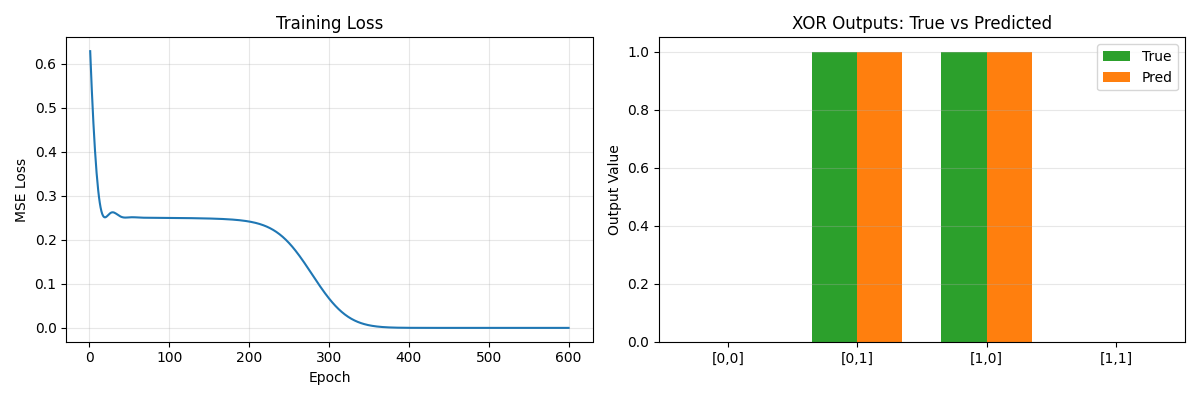
\includegraphics[width=0.92\textwidth]{output.png}
		\caption{训练损失曲线与 XOR 预测结果对比}
	\end{figure}
	
	\section*{七、实验总结}
	在本次实验中，我们实现了前馈神经网络最基本的架构：数据输入、网络搭建、前向传播、损失计算、反向传播、参数更新以及结果可视化。并直观的感受神经网络在分类问题的强大之处。另外，我们将数据具体化，以数据体现隐藏层的作用。
	
\end{document}
